\documentclass[conference]{IEEEtran}
%+++++++++++++++++++++++++++++++++++++++++++
% Added to commands
\input epsf
\usepackage{graphicx}
\usepackage{subcaption}
\usepackage [french]{babel}
\usepackage [utf8]{inputenc}
\usepackage [T1] {fontenc}
\usepackage{float}
%+++++++++++++++++++++++++++++++++++++++++++
% correct bad hyphenation here
\hyphenation{op-tical net-works semi-conduc-tor IEEEtran}
\begin{document}

%+++++++++++++++++++++++++++++++++++++++++++
\title{\LARGE Etude de la VSM pour la simulation de LEI kites
\vskip10pt

\small 2024 - Romain LAMBERT
}
%+++++++++++++++++++++++++++++++++++++++++++
% make the title area
\maketitle

\begin{abstract}Ce bureau d'étude a pour sujet l'étude de la VSM. L'objectif final étant de déterminer l'intérêt de la VSM pour nos simulation numériques. 
\end{abstract}
\IEEEoverridecommandlockouts

\IEEEpeerreviewmaketitle
\section{VSM vs VLM }

\subsection{\textbf{ChatGPT}} 

\begin{table}[h!]
    \centering
    \begin{tabular}{|l|c|c|}
    \hline
    \textbf{Aspect}                  & \textbf{Vortex Lattice Method (VLM)}              & \textbf{Vortex Step Method (VSM)}               \\ \hline
    \textbf{Modélisation}            & Grille de panneaux avec vortex sur la surface     & Tourbillons libres évoluant dans le temps       \\ \hline
    \textbf{Régime}                  & Stationnaire (analyse aérodynamique stable)       & Instationnaire (analyse des mouvements transitoires) \\ \hline
    \textbf{Charge de calcul}        & Relativement faible                               & Plus élevée (calculs temporels)                 \\ \hline
    \textbf{Applications typiques}   & Ailes d’avion, surfaces fixes                     & Ailes battantes, simulations transitoires complexes \\ \hline
    \textbf{Résolution}              & Problème de potentiel stationnaire                & Suivi temporel des vortex libres                \\ \hline
    \end{tabular}
    \caption{Comparaison entre la Vortex Lattice Method et la Vortex Step Method}
    \end{table}
    
En conclusion, la \textbf{Vortex Lattice Method} est souvent utilisée pour des analyses stationnaires d'ailes fixes, tandis que la \textbf{Vortex Step Method} est adaptée pour les écoulements instationnaires, où les tourbillons évoluent dynamiquement dans le temps.

\subsection{\textbf{Ocayon - Delft}} 
Il existe 3 méthodes basses fidélités pour les flux potentiels : LLT, VLM, VSM.

La LLT ne fonctionnne pas très bien pour les géométries non conventionnelles (dihèdre, flèche, ...). La VSM résoud ce problème avec un temps de calcul égal.

Là où la VLM semble être l'application discrète de la LLT (méthode des panneaux), la VSM semble diverger de la VLM par sa prise en compte des effets 3D du décrochage. Telle une simulation RANS, la VSM converge pour des cas insationnnaires (décrochage) en itérant sur la loi de circulation. \\

Voici les grandes lignes de la théories derrière la VSM : \\

\textbf{Hypothèses} \\
\begin{itemize}
    \item L'écoulement peut être divisé en deux régions : la région interne et la région externe. D'une part, l'écoulement dans la région interne représente les propriétés du profil aérodynamique, qui peuvent être obtenues par une variété de méthodes. D'autre part, l'écoulement en dehors de la région du profil est sans viscosité, irrotationnel et incompressible, afin d'obtenir une solution d'écoulement potentiel.
    \item Le théorème de Kutta–Joukowski est satisfait dans chaque section de l'aile, reliant les régions interne et externe.
    \item L'écoulement est quasi-stationnaire, ce qui signifie que chaque condition d'écoulement peut être résolue uniquement dans le domaine spatial.
    \item Le vortex de départ est situé très en aval et son influence peut être négligée.
    \item HYPOTHÈSE DU SILLAGE FIGÉ.
\end{itemize}

\textbf{Système de vorticity}
\begin{figure}[H]
    \centering
    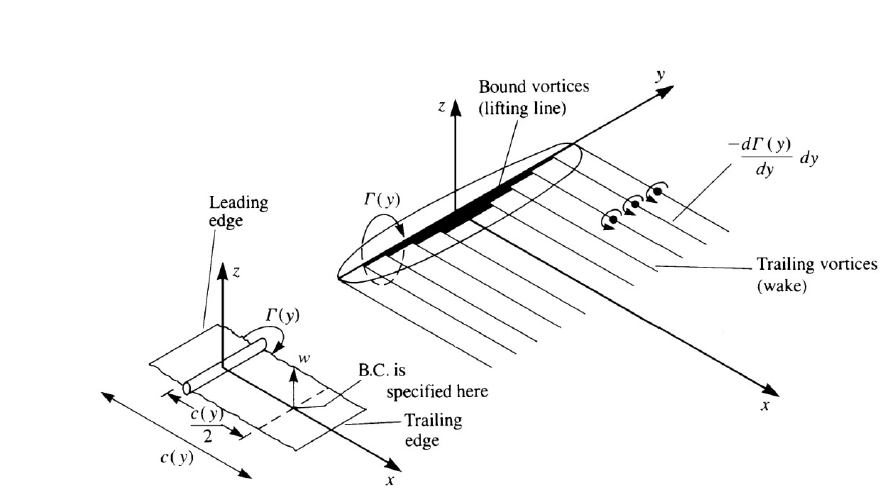
\includegraphics[width=0.7\textwidth]{Pics/vortex VSM.png}
    \caption{Représentation du modèle de ligne portante constitué de tourbillons en fer à cheval}
    \label{fig: vortex vsm}
\end{figure}


Dans la théorie classique de la ligne portante de Prandtl, la ligne portante est supposée être droite, et les tourbillons traînants sont uniquement responsables de l'induction du vent induit qui modifie les angles d'attaque locaux. En revanche, dans un cas plus général, où la ligne portante n'est pas droite, comme dans le cas du VSM actuellement étudié, l'ensemble du système de vorticité joue un rôle dans le changement de l'angle d'attaque sectionnel.\\

\begin{figure}[H]
    \centering
    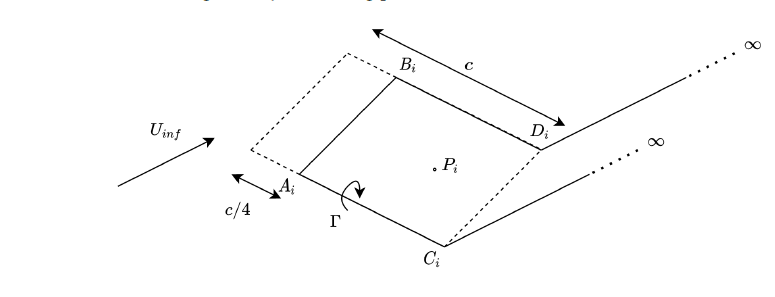
\includegraphics[width=0.7\textwidth]{Pics/Panneaux VSM.png}
    \caption{Représentation de la géométrie d'un vortex en fer à cheval}
    \label{fig:panneau vsm}
\end{figure}

\textbf{Les vitesses induites des panneaux J sur les points de control i}

Ces vitesses induites sont compliquées à exprimer selon si on se situe sur un panneaux ou un filament infinie. La formule générale est la suivante : 
\begin{equation}
    dw = \frac{\Gamma}{4 \pi} \frac{dl x r}{|r|^3}
\end{equation}

\textbf{Matrice d'influence AIC}

Ainsi on lie vitesse induite en un point de control i par l'ensemble des circulations $\Gamma$ des panneaux j via des matrices d'influences : 
\begin{equation}
    u = AIC_u \Gamma
    \label{eq:gamma}
\end{equation}

\textbf{Calcul de la circulation}
\begin{equation}
    \rho |U_{\infty} \Gamma_j| - \frac{1}{2} \rho |U_{rel} z_{airf}|^2 c C_l(\alpha_{EFF_j}) = 0
    \label{eq:gamma_new}
\end{equation}

\textbf{Résolution par itération à convergence}\\
On part d'une circulation $\Gamma$ initiale, on en déduit la vitesse induite (eq. \ref{eq:gamma}), on calcul l'angle induit ($\alpha_{tot} = \alpha + \alpha_{ind}$), on calcul $C_l(\alpha)$ (ici, avec le code de Ocaryon, on utilise la formule de régression de Breukels), puis on calcul à nouveau $\Gamma$ grâce à l'équation \ref{eq:gamma_new}. On itère le procédé jusqu'à convergence...

%%%%%%%%%%%%%%%%%%%%%%%%%%%%%%%%%%%%%%%%%%%%%%%%%%%%%%%%%%%%%%%%%%%%%%%%%%%%%%%%%%

\IEEEpeerreviewmaketitle
\section{Test VSM/VLM sur SeaKite $50m^2$ VH}

\subsection{Polaires Sur l'aile de DELFT} 

\begin{figure}[H]
    \centering
    \begin{subfigure}[b]{0.45\textwidth}
        \centering
        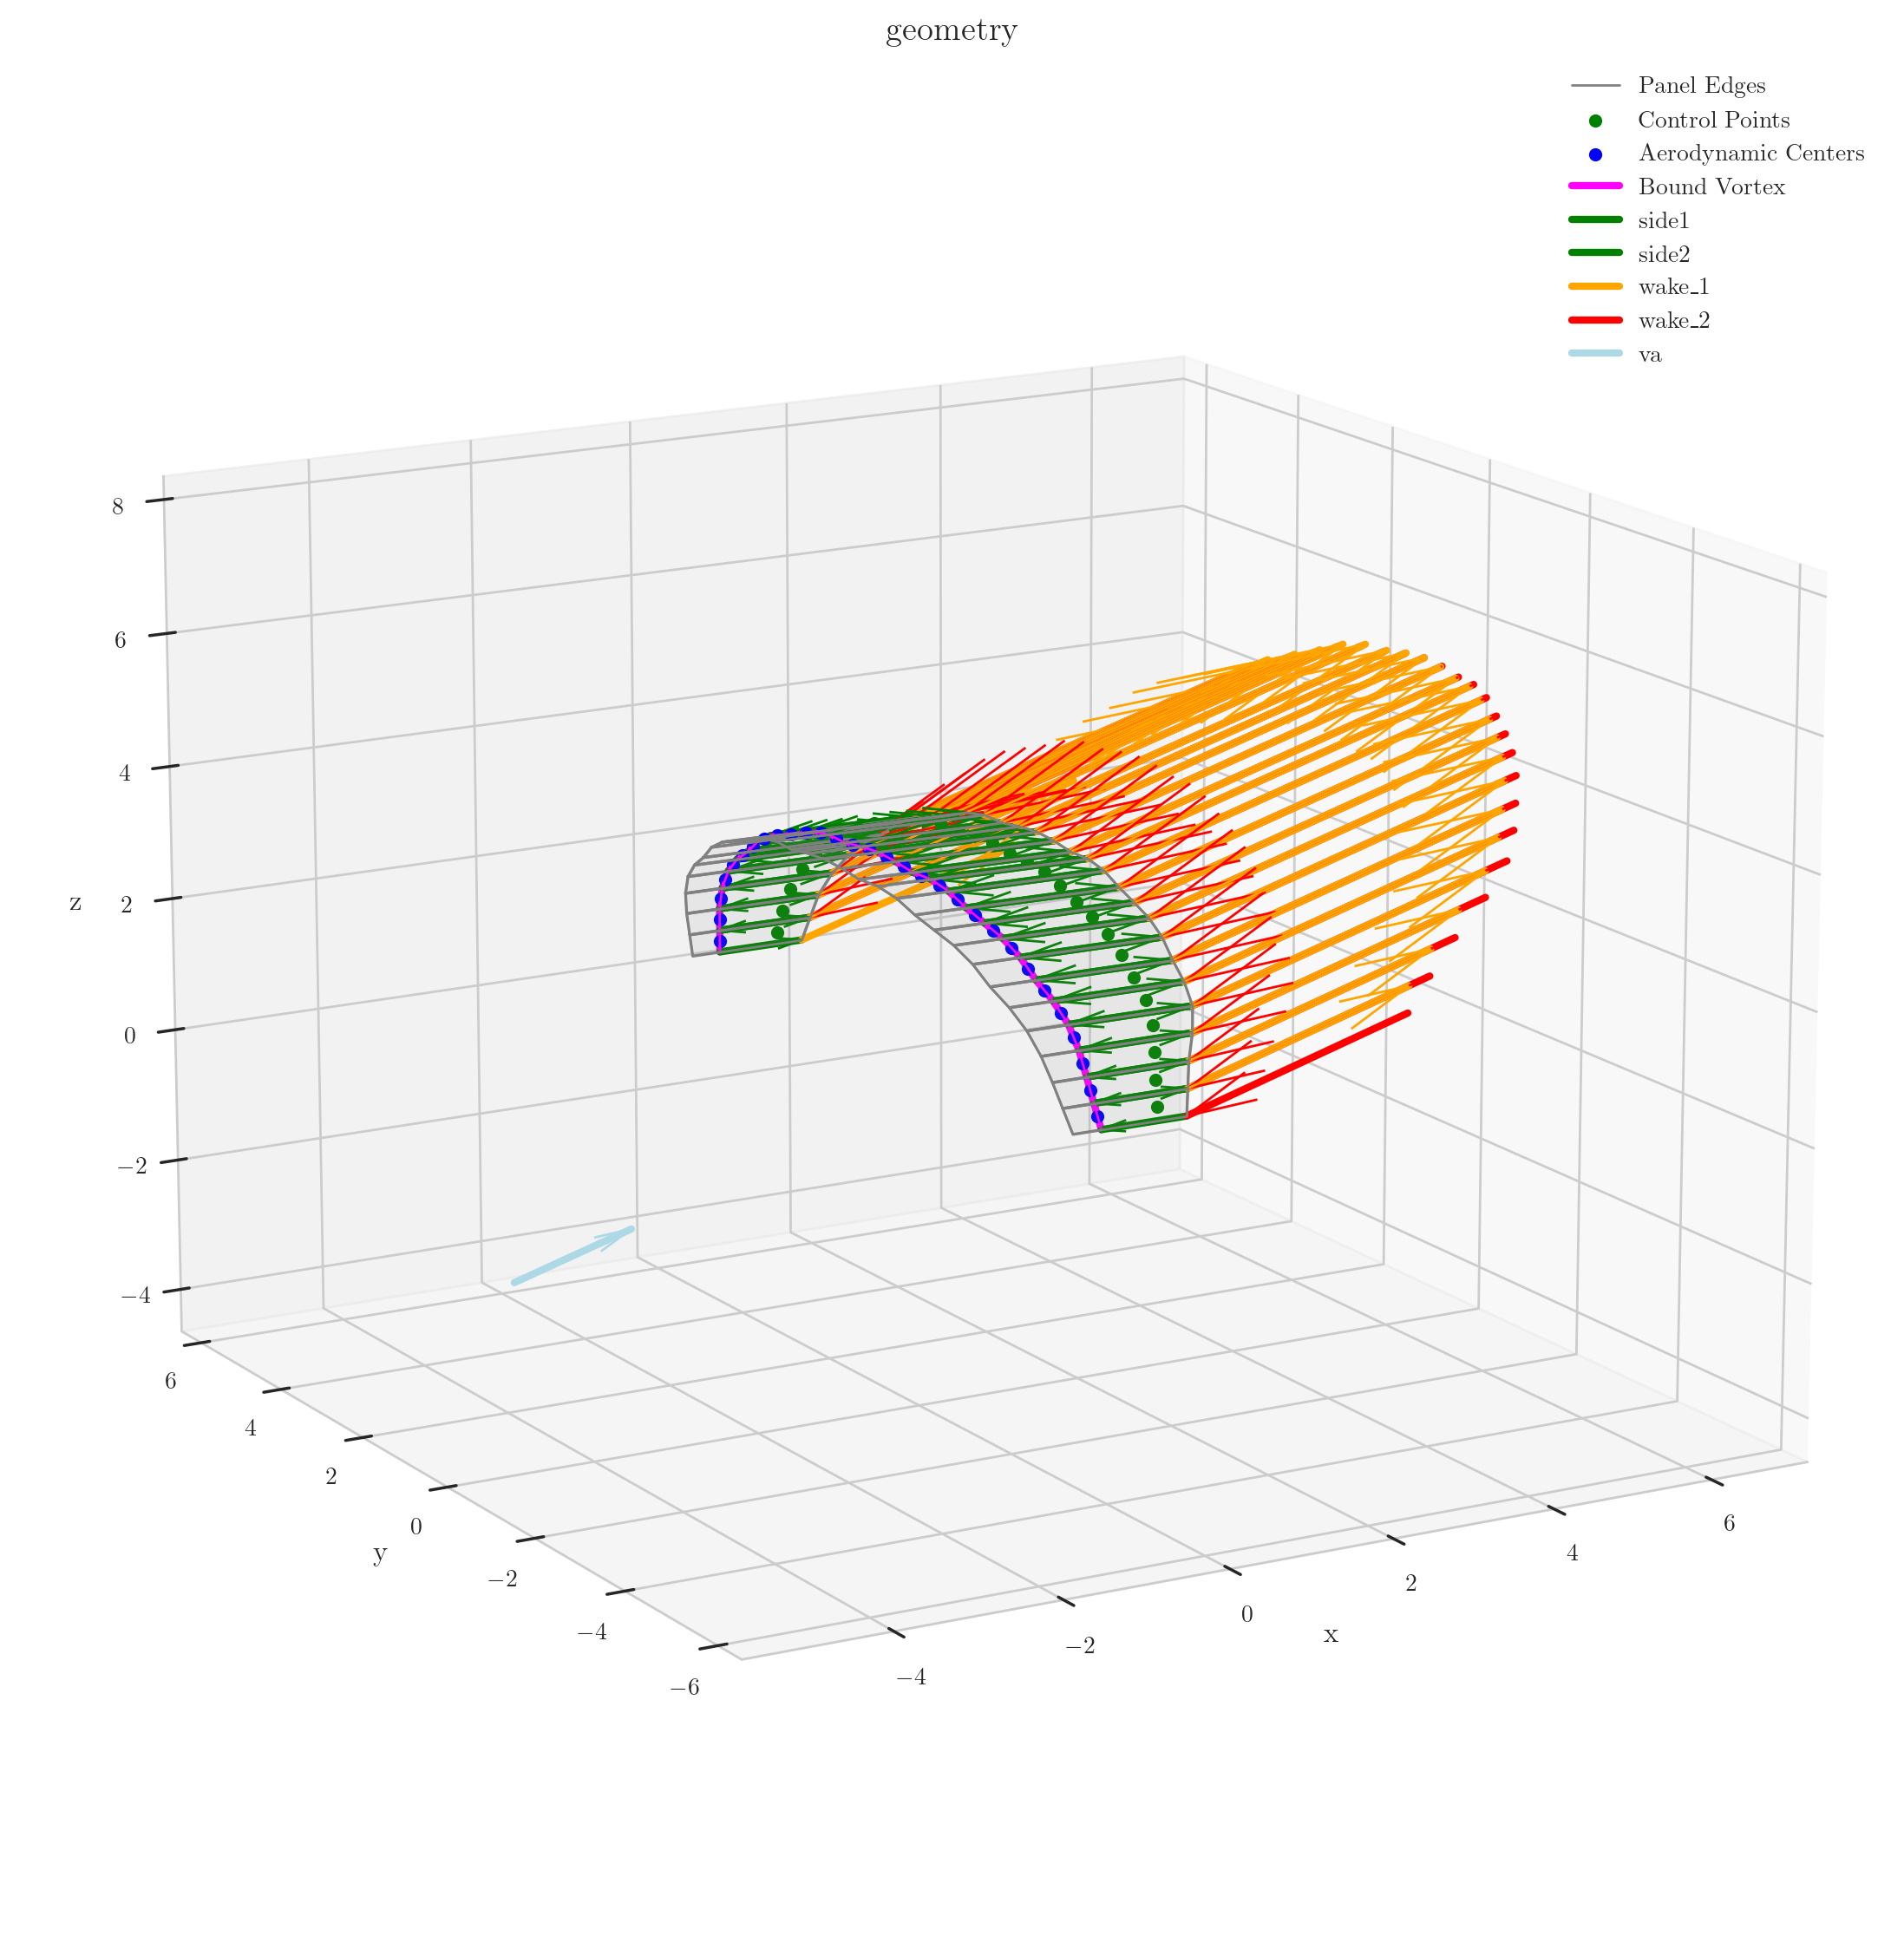
\includegraphics[width=\textwidth]{Pics/kite delft vsm.png}
        \caption{Kite de Delft tel que modélisé par la VSM}
        \label{fig:Kite de Delft tel que modélisé par la VSM}
    \end{subfigure}
    \hfill
    \begin{subfigure}[b]{0.45\textwidth}
        \centering
        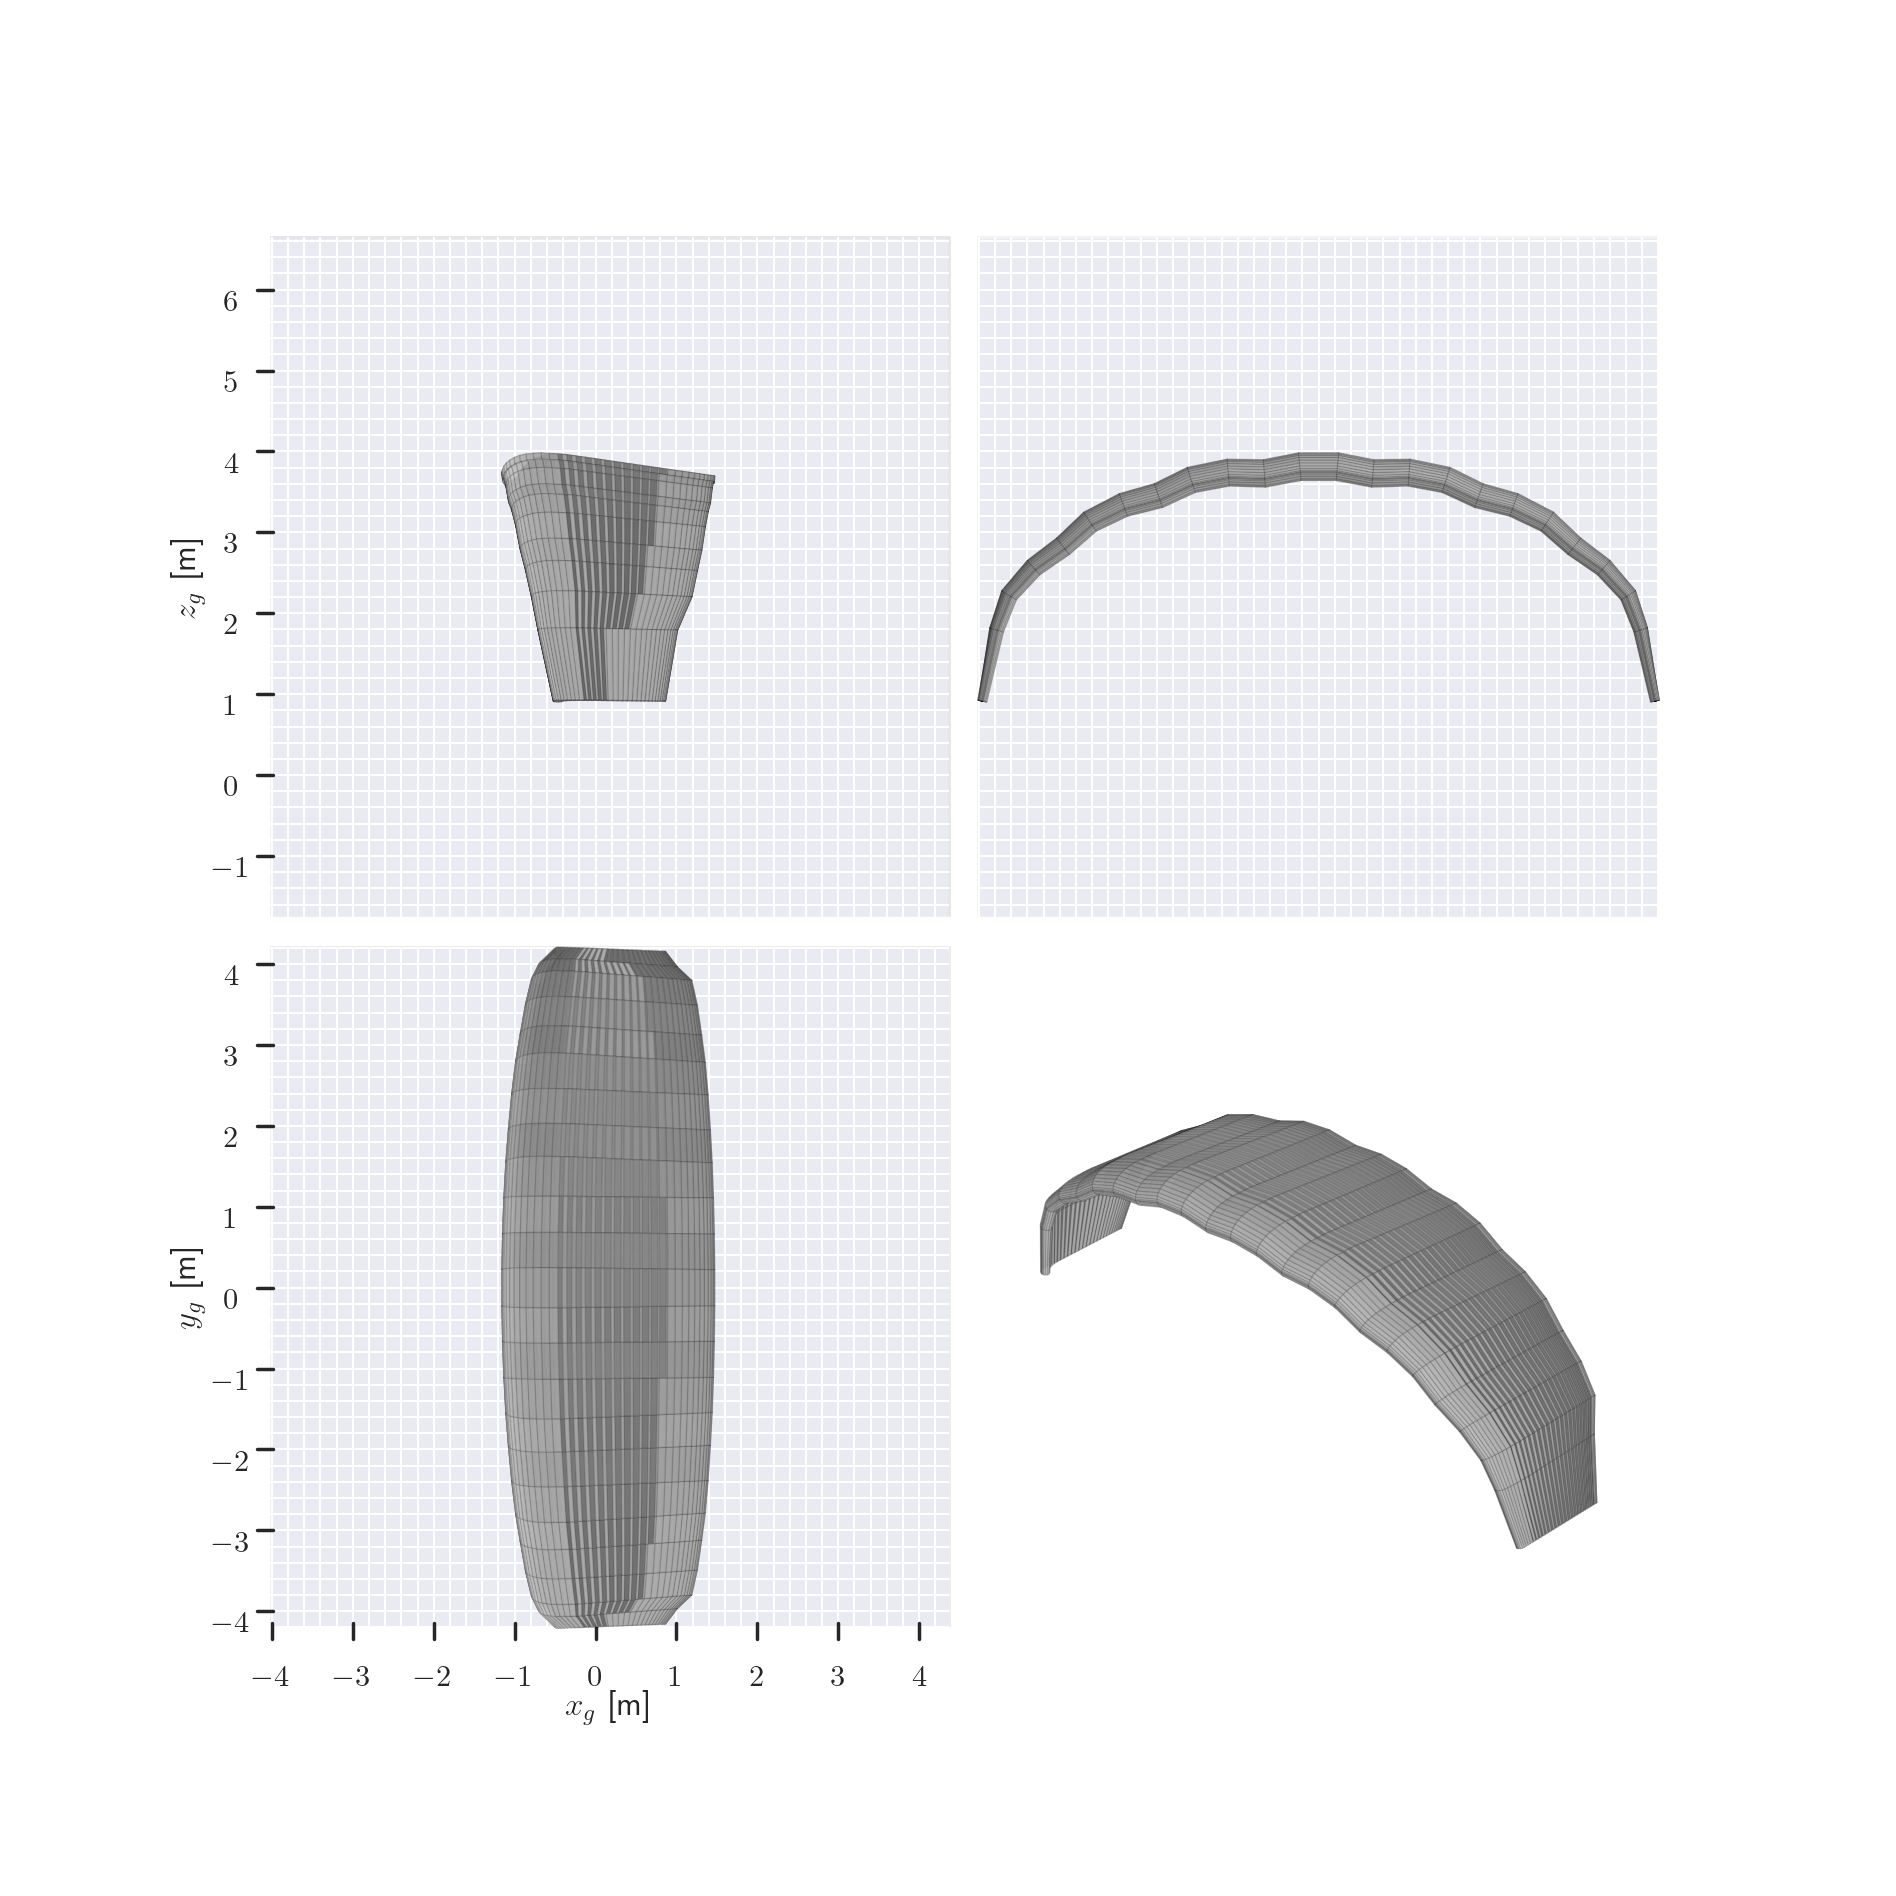
\includegraphics[width=\textwidth]{Pics/kite delft vlm.png}
        \caption{Kite de Delft tel que modélisé par la VLM}
        \label{fig:Kite de Delft tel que modélisé par la VLM}
    \end{subfigure}
    \caption{Deux graphiques côte à côte}
    \label{fig:deux_graphiques}
\end{figure}

\begin{figure}[H]
    \centering
    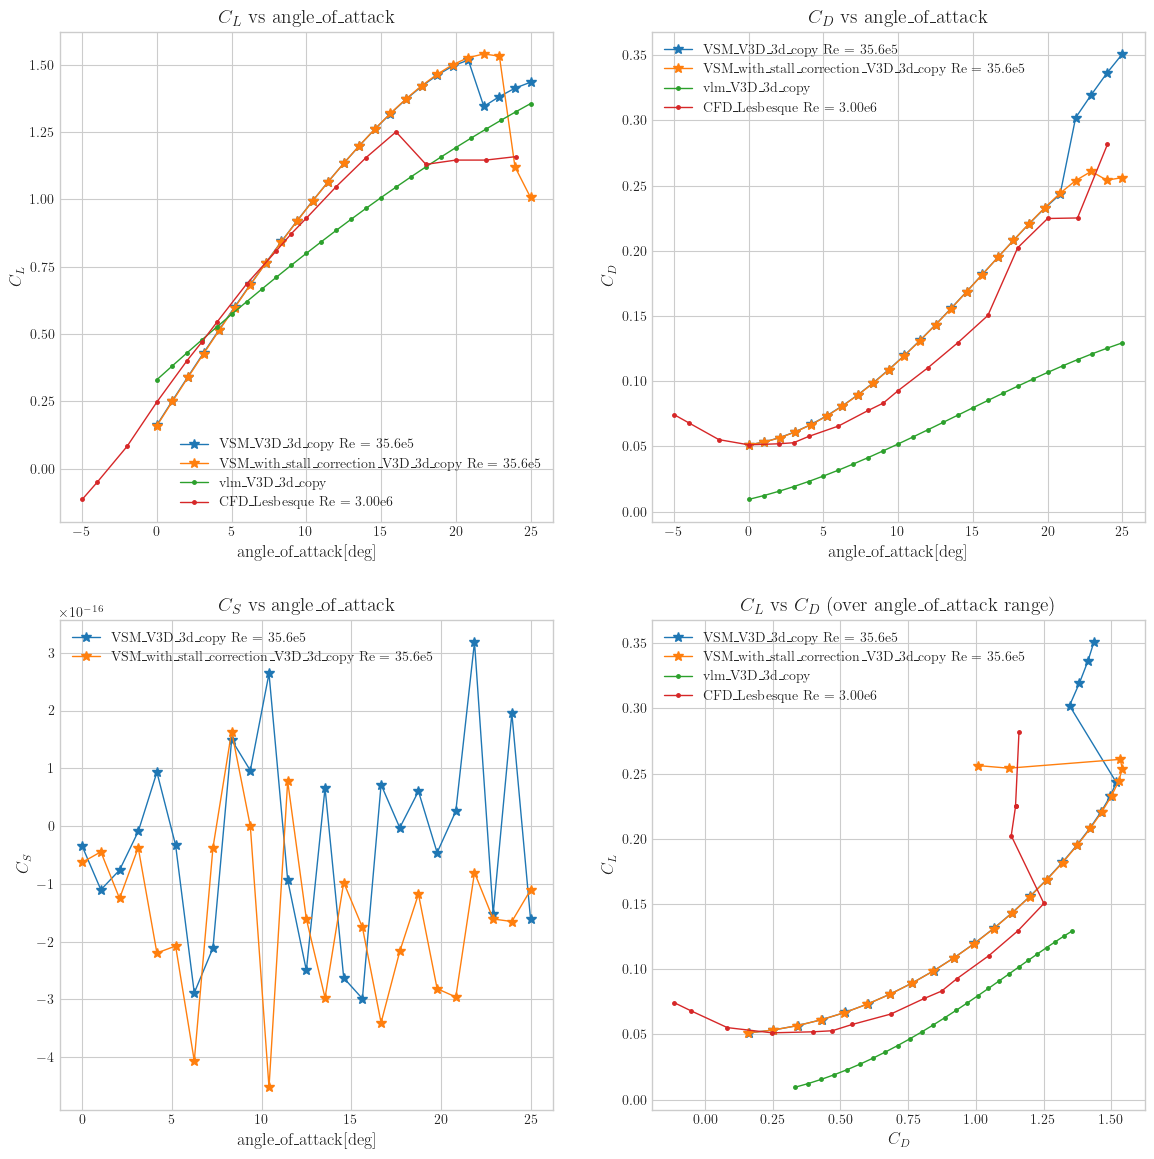
\includegraphics[width=0.7\textwidth]{Pics/polar delft.png}
    \caption{Comparatif des polaires pour l'aile de DELFT}
    \label{fig:Comparatif des polaires pour l'aile de DELFT}
\end{figure}

\begin{figure}[H]
    \centering
    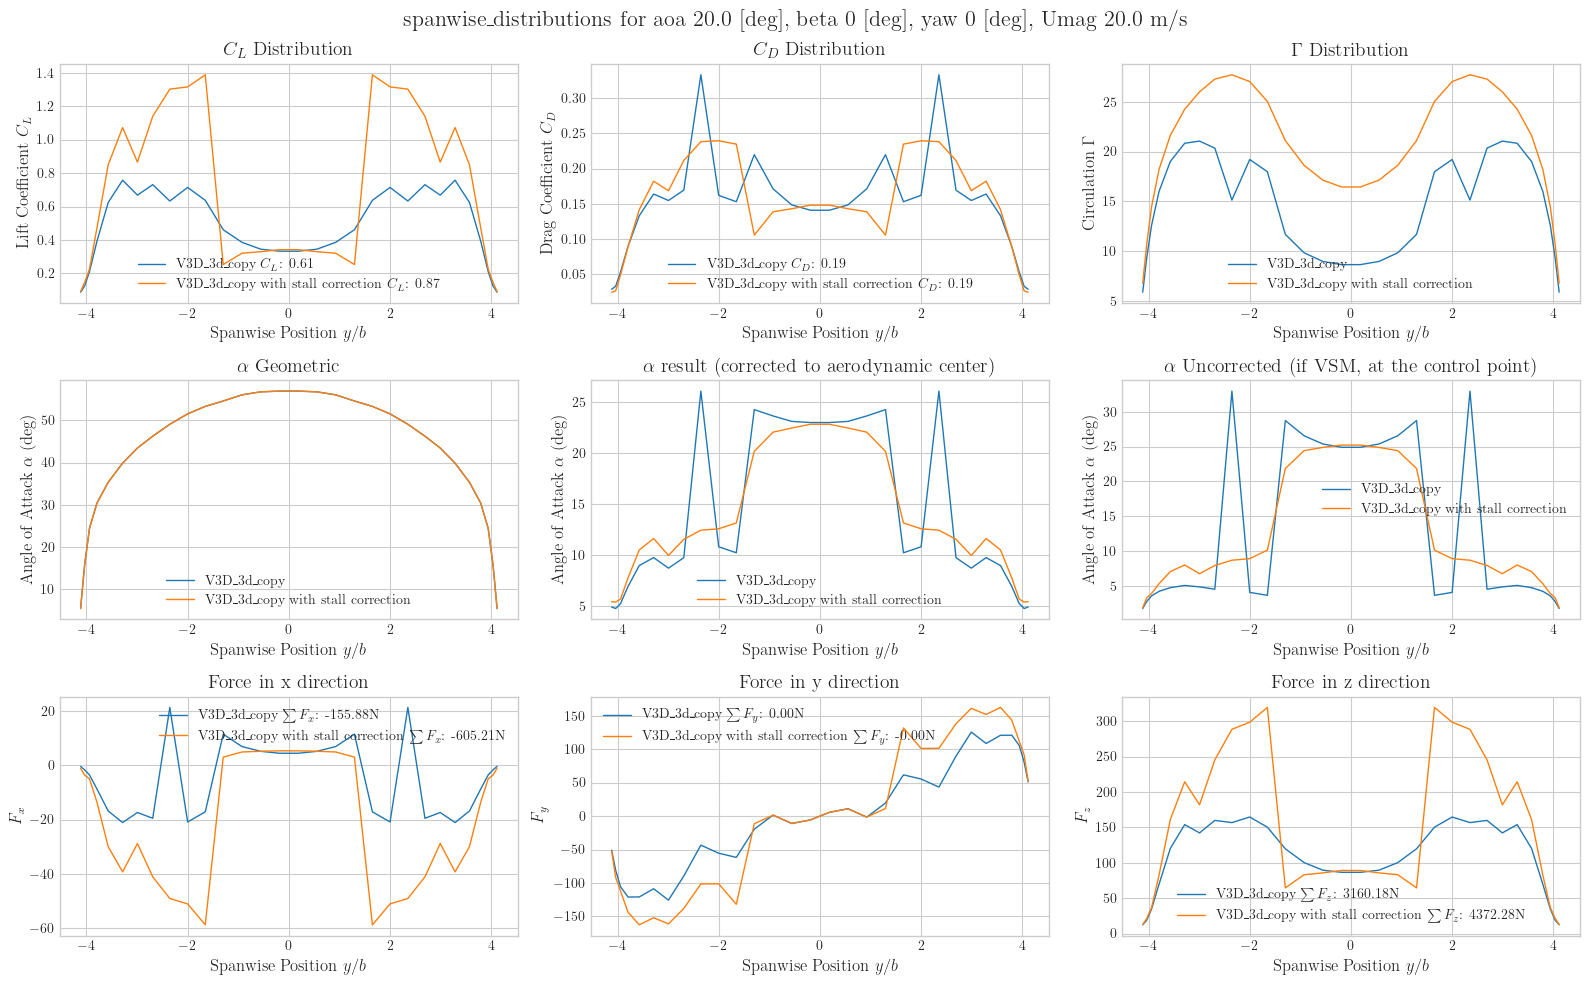
\includegraphics[width=0.7\textwidth]{Pics/circulation DELFT.png}
    \caption{Comparatif des circulation pour l'aile de DELFT}
    \label{fig:Comparatif des circulation pour l'aile de DELFT}
\end{figure}


\subsection{Polaires Sur l'aile de BEYOND} 

\begin{figure}[H]
    \centering
    \begin{subfigure}[b]{0.45\textwidth}
        \centering
        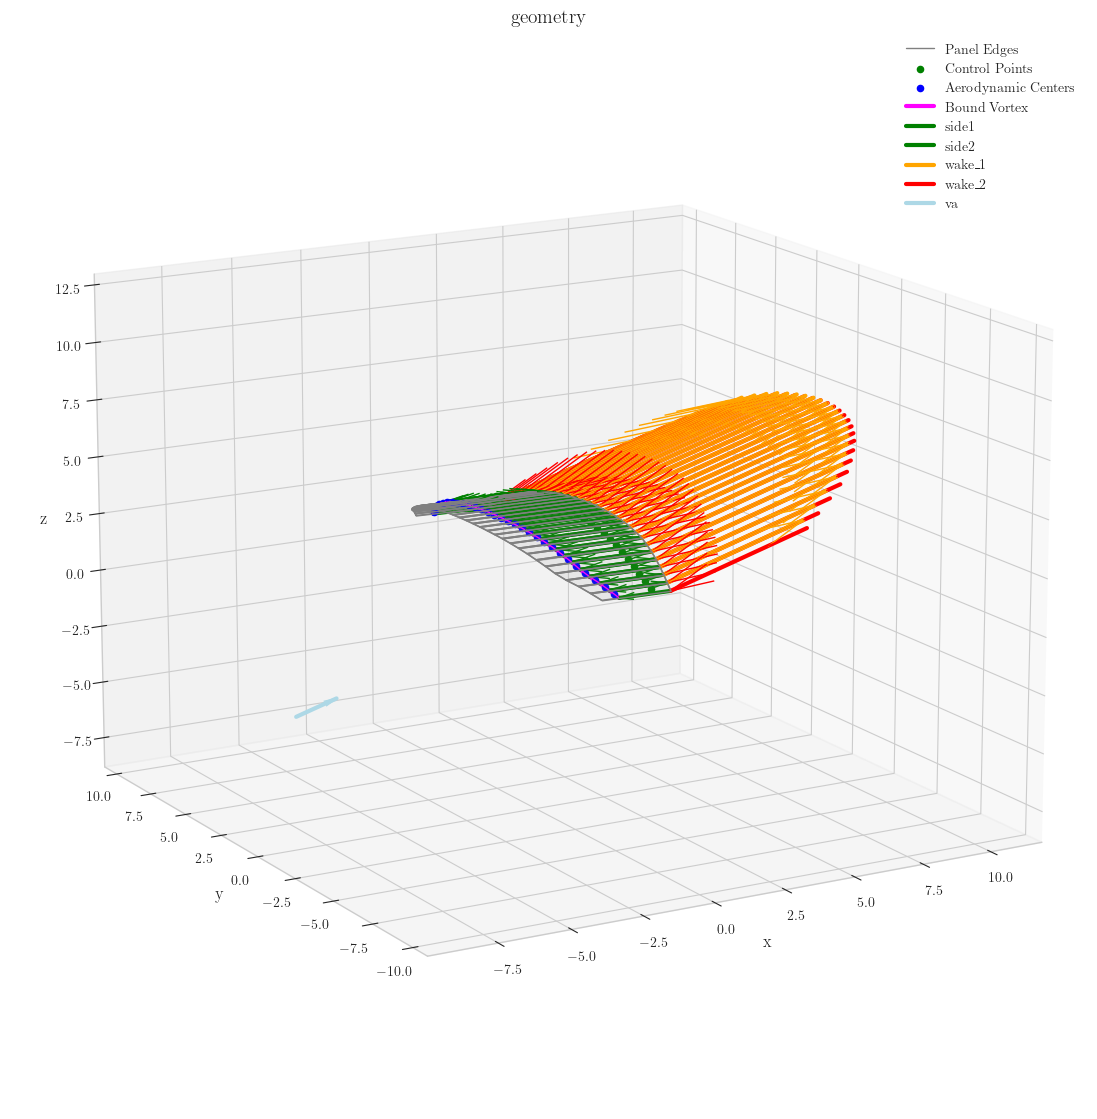
\includegraphics[width=\textwidth]{Pics/kite beyond vsm.png}
        \caption{Kite de Beyond tel que modélisé par la VSM}
        \label{fig:Kite de Beyond tel que modélisé par la VSM}
    \end{subfigure}
    \hfill
    \begin{subfigure}[b]{0.45\textwidth}
        \centering
        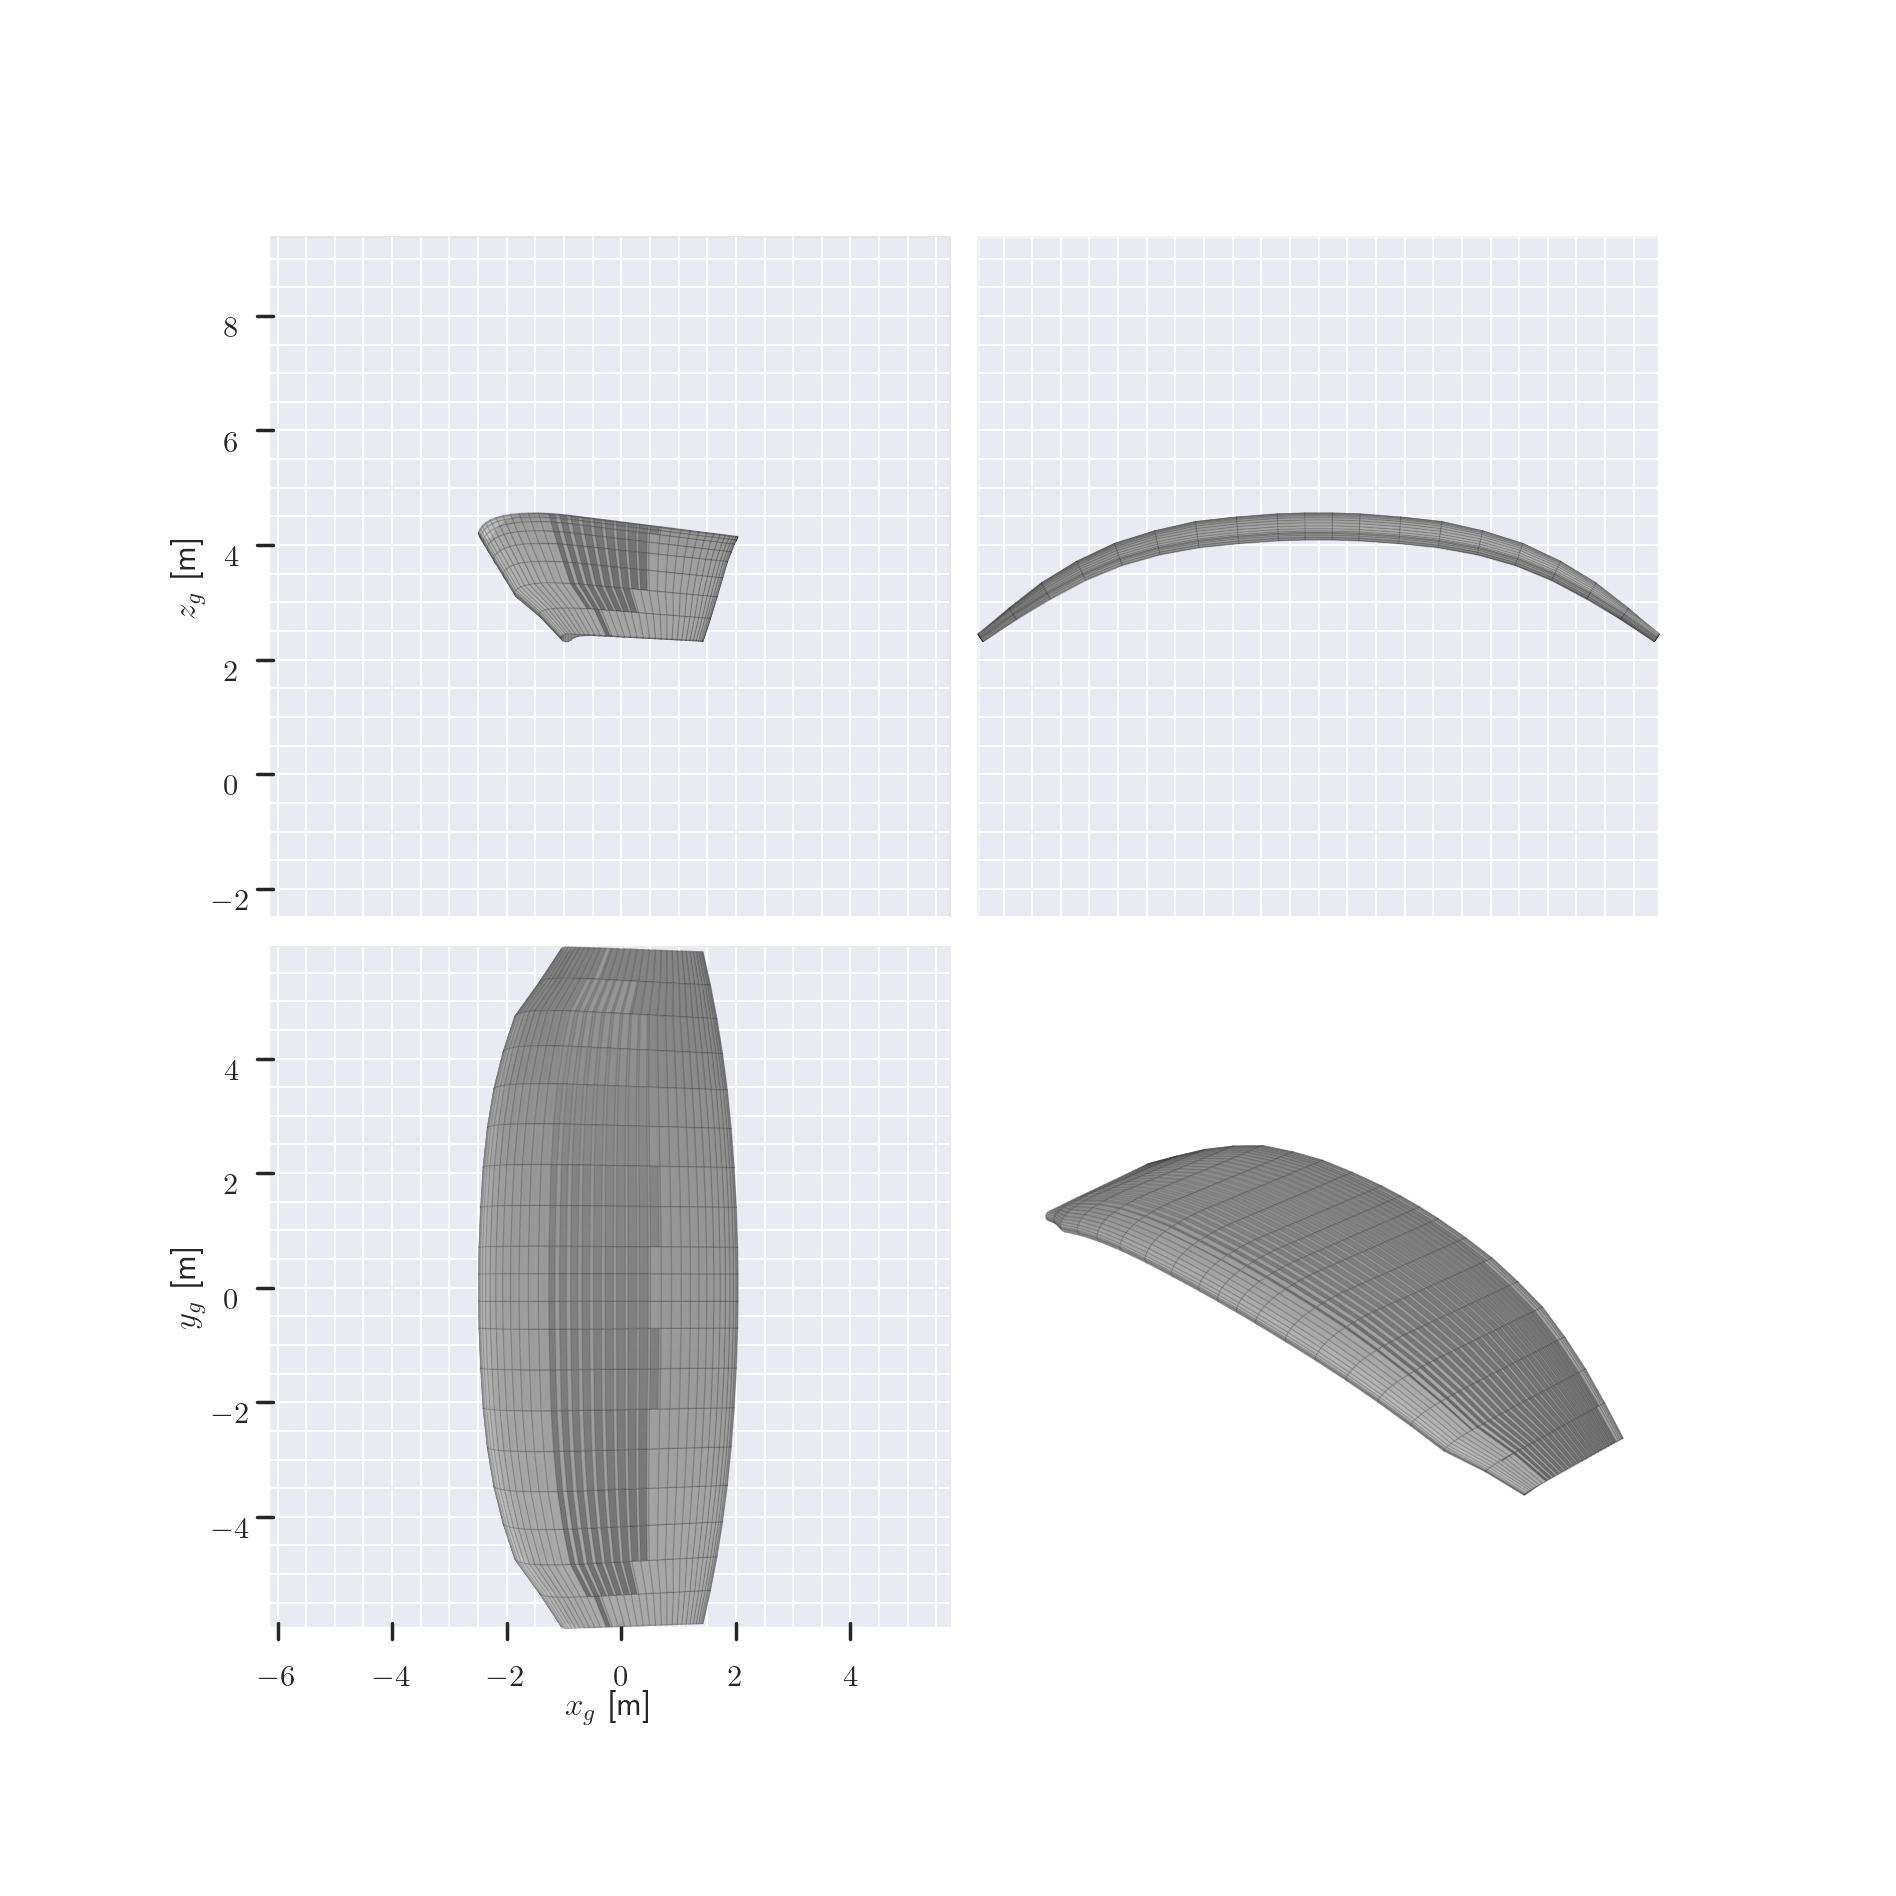
\includegraphics[width=\textwidth]{Pics/kite beyond vlm.png}
        \caption{Kite de Beyond tel que modélisé par la VLM}
        \label{fig:Kite de Beyond tel que modélisé par la VLM}
    \end{subfigure}
    \caption{Deux graphiques côte à côte}
    \label{fig:deux_graphiques}
\end{figure}

\begin{figure}[H]
    \centering
    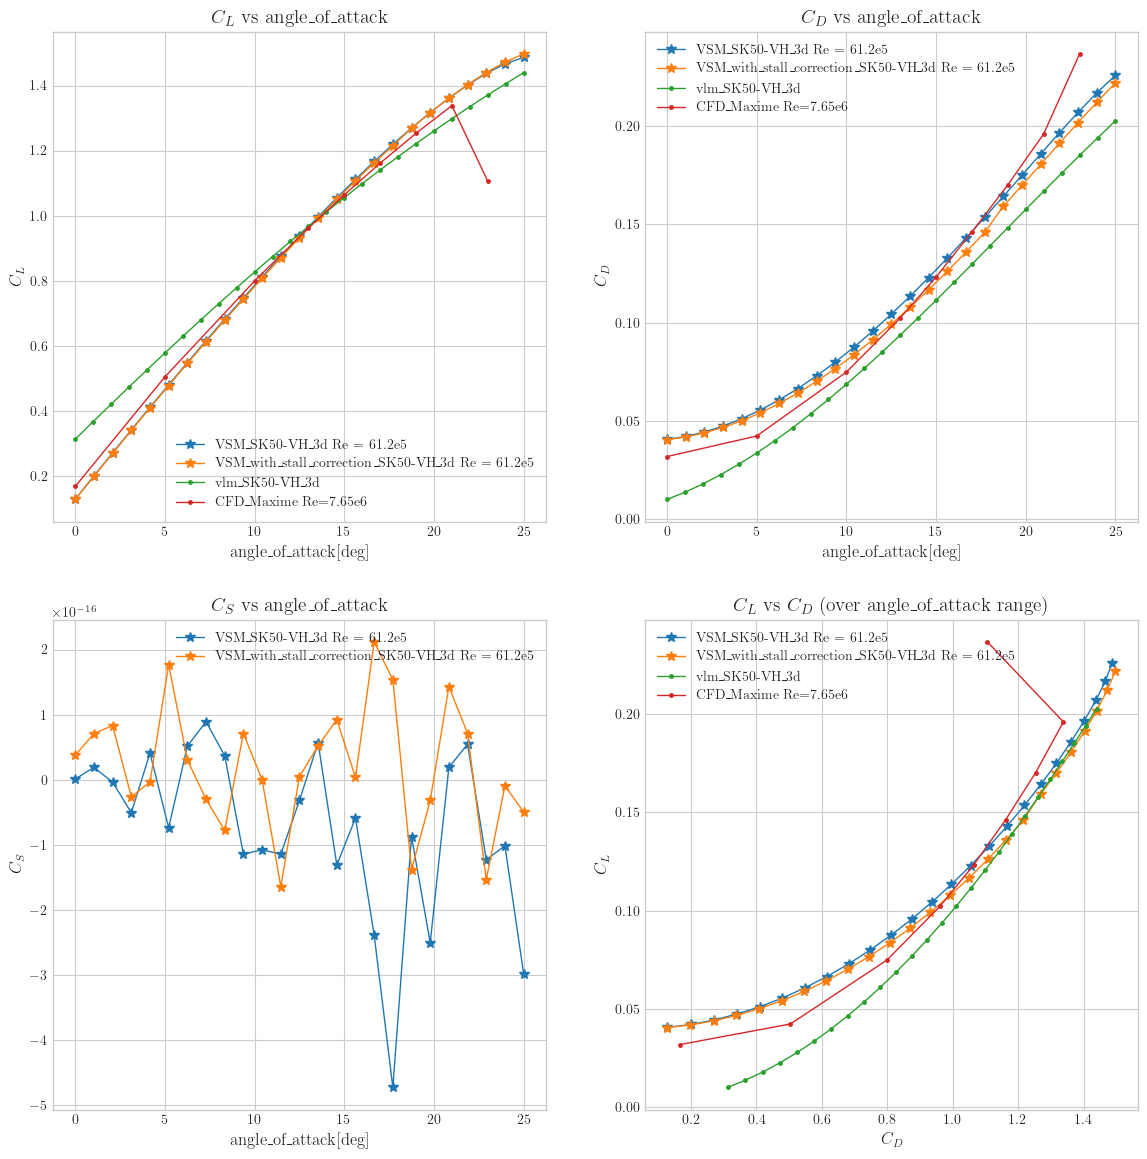
\includegraphics[width=0.7\textwidth]{Pics/polar BEYOND.png}
    \caption{Comparatif des polaires pour l'aile de BEYOND}
    \label{fig:Comparatif des polaires pour l'aile de BEYOND}
\end{figure}

\begin{figure}[H]
    \centering
    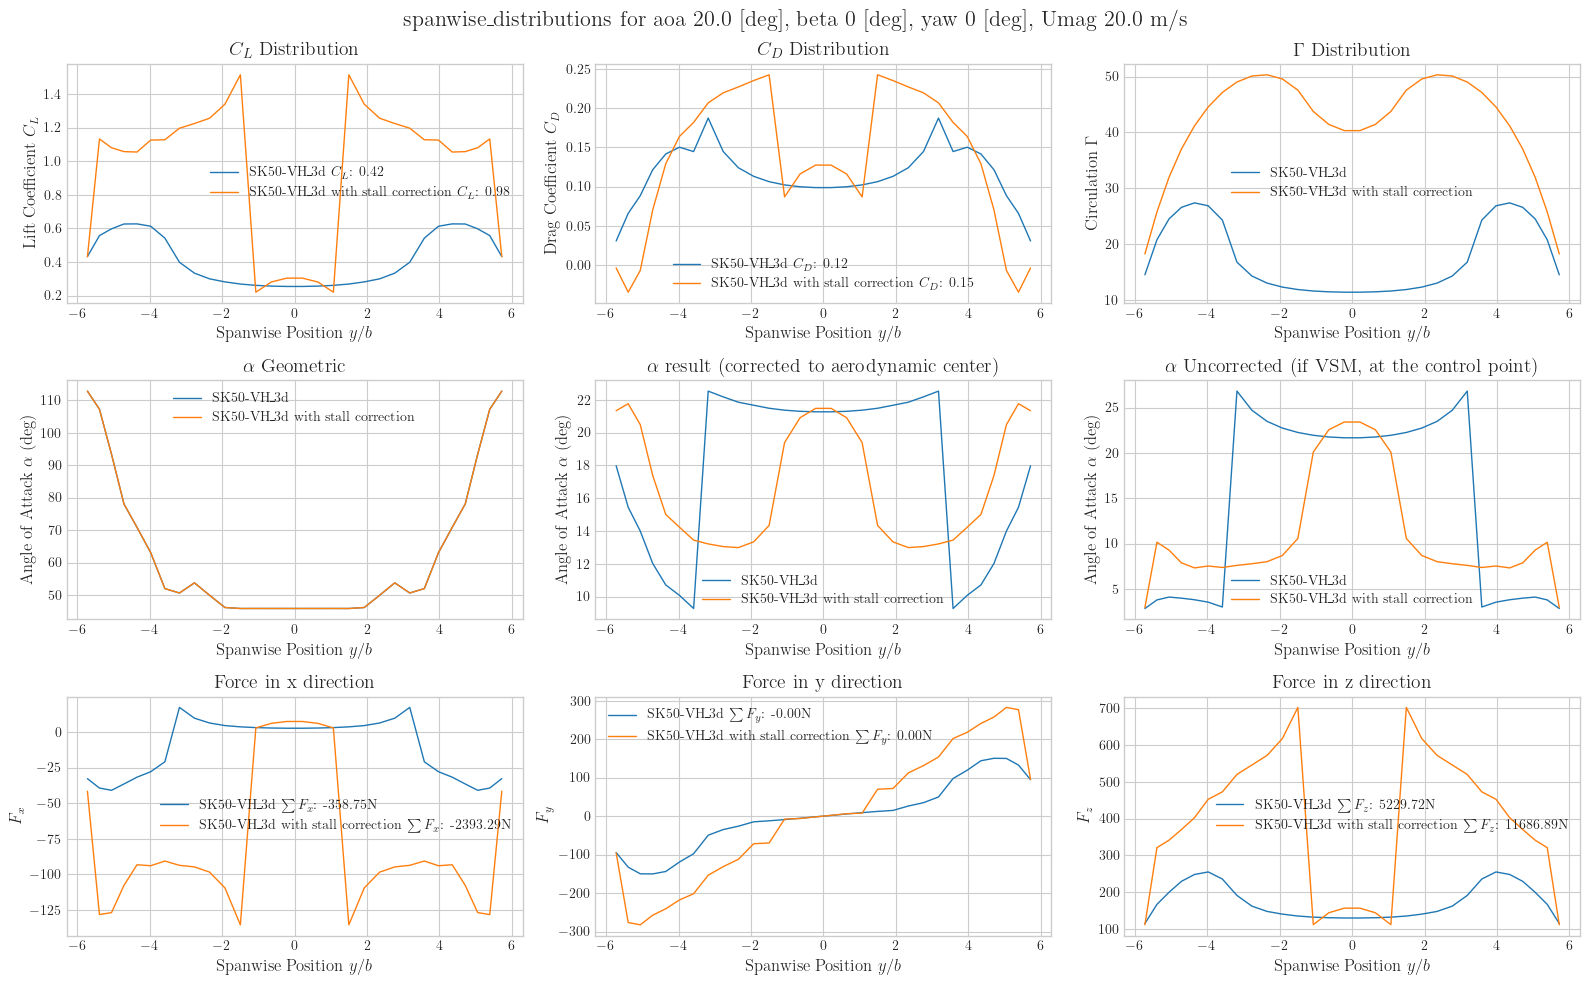
\includegraphics[width=0.7\textwidth]{Pics/circulation BEYOND.png}
    \caption{Comparatif des circulation pour l'aile de BEYOND}
    \label{fig:Comparatif des circulation pour l'aile de BEYOND}
\end{figure}

\subsection{Analyse} 

Pour le moment VLM est VSM semble proche des résultats obtenus par CFD. \\
On remarque que, dans le cas de la voile de Delft, la VSM semble capturer un effet de décrochage là où la VLM ne le prend pas en compte (résultat attendu).\\
Les résultats de la VLM sont moins concluant pour la voile de Delft \textbf{mais} la 3d associé présente des défauts qui pourraient expliquer ce décalage... \\

\textbf{TODO} :
\begin{itemize}
    \item Améliorer la géométrie de l'aile pour la VLM
    \item Afficher la répartition de circulation en envergure pour la VLM afin de la comparer à celle de la VSM
    \item Utiliser de l'optim sur la VLM (car Aerosandbox le permet)
\end{itemize}

\end{document}